\documentclass[10pt,a4paper]{article}
\usepackage[latin1]{inputenc}
\usepackage{amsmath}
\usepackage{amsfonts}
\usepackage{amssymb}
\usepackage{graphicx}
\usepackage{hyperref}
\usepackage{float}
\begin{document}
\title{Usage Modelling\\scalability iobserve-analysis}
\date{}
\maketitle

\section{General}
\textbf{Code:} \url{https://github.com/research-iobserve/iobserve-analysis/tree/scalability-usability-1}\\
\textbf{Test data and results:} \url{https://github.com/research-iobserve/iobserve-analysis/tree/scalability-usability-1/tests/scalability_test_setup}

\section{Set ups:}
Each of the described setups is run 10 times and the results are averaged.

\subsection{equal\_events\_x\_users:}
The same call executed from X users successively. The executed call has the following signature:\\ \emph{org.cocome.cloud.logic.webservice.cashdeskline.cashdesk.CashDesk.startSale(java.lang.String,long)}

\subsection{x\_different\_events\_one\_user:}
A single user executing X calls successively. The testdata is made up of randomly created sequences of calls taken from the CoCoMe case study, which have a direct mapping from monitoring data to the pcm model instance. The call signatures are the following:
\emph{{\tiny
		\begin{itemize}
			\item org.cocome.cloud.logic.webservice.cashdeskline.cashdesk.barcodescanner.BarcodeScanner.sendProductBarcode(java.lang.String,long,long)
			\item org.cocome.cloud.logic.webservice.cashdeskline.cashdesk.CashDesk.startSale(java.lang.String,long)
			\item org.cocome.cloud.logic.webservice.cashdeskline.cashdesk.CashDesk.selectPaymentMode(java.lang.String,long,java.lang.String)
			\item org.cocome.cloud.logic.webservice.cashdeskline.cashdesk.CashDesk.finishSale(java.lang.String,long)
			\item org.cocome.cloud.logic.webservice.store.StoreManager.createStockItem(long,org.cocome.tradingsystem.inventory.application.store.ProductWithStockItemTO)
			\item org.cocome.tradingsystem.inventory.application.store.StoreServer.getProductWithStockItem(long,long)
			\item org.cocome.tradingsystem.inventory.application.store.StoreServer.getStore(long)
			\item org.cocome.tradingsystem.inventory.data.enterprise.StoreEnterpriseQueryProvider.queryEnterpriseByName(java.lang.String)
			\item org.cocome.tradingsystem.inventory.data.enterprise.TradingEnterprise.initTradingEnterprise()
			\item org.cocome.tradingsystem.inventory.data.store.EnterpriseStoreQueryProvider.queryStockItem(long,long)
			\item org.cocome.tradingsystem.inventory.data.store.EnterpriseStoreQueryProvider.queryStoreById(long)
			\item org.cocome.tradingsystem.inventory.data.store.Store.initStore()
			\item org.cocome.tradingsystem.inventory.data.store.StoreDatatypesFactory.fillStoreWithEnterpriseTO(org.cocome.tradingsystem.inventory.data.store.IStore)
\end{itemize}}}
Due to the very limited amount of different calls and random creation of call sequences, some successive sections may be identical, or may only be made up of the same successive call, resulting in loops and branches in the created UsageModel.

\section{TPreprocess}
The TPreprocess filter is an abstract superordinate filter, which preprocesses the incoming monitoring data. It actually is made up of two connected sub filters:

\paragraph{TEntryCall}
Monitoring data regarded by this evaluation setups is made up of three types of records. Each call starts with a TraceMetadata record, followed by a BeforeOperationObjectEvent and a corresponding AfterOperationObjectEvent. Together, these three records represent a single call from one user session. Records that are related, because they are from the same user session carry an identical session id and call id. TEntryCall filters and maps these related records, to recreate calls which are present in the monitoring data. Once an AfterOperationObjectEvent is mapped to a previously processed BeforeOperationObjectEvent, an EntryCallEvent representing the call is forwarded to TEntryCallSequence. This is nesseccary, as in normal monitoring data it would be is possible, that there is an arbitrary amount records from other sessions between three related ones.\\
\\
TEntryCall only operates on HashMaps, which results in a time complexity of $\mathbf{O(1)}$

\paragraph{TEntryCallSequence}
While TEntryCall recreates calls, TEntryCallSequence maps the incoming EntryCallEvents according to their session id, recreating user sessions. All sessions that exceed a certain size are collected and used to create a new EntryCallSequenceModel, which is then forwarded. \\
Only events which have a direct mapping to a PCM entity can be considered in the further process. To ensure this, the CorrespondenceModel is used to check if a correspondance exists for each incoming EntryCallEvent. This operation relies on parsing the class and operation signatures of the EntryCallEvent two times, which results in a time complexity of $\mathbf{O(2 * c + 2 * o)}$, for the first occurrence of each call. For following occurrences of similar calls, with an equal class and operation signature, the time complexity drops to $\mathbf{O(c + o)}$. This is due to correspondences being mapped in a HashMap once they occur, removing the need to parse the class and operation signature a second time.\\
\\
Combining TEntryCall and TEntryCallSequence results in a big O notation time complexity of $\mathbf{O(c + o)}$, for \textbf{single run} of TPreprocess. In each of the evaluation setups the TPreprocess filter is called $\mathbf{mc}$ times, where mc is the amount of monitored calls in the monitoring data.\\
\\
This results in a \textbf{overall} time complexity of $\mathbf{O(mc * (c + o))}$ \\
c = length of class signature in monitoring data\\
o = length of operation signature in monitoring data\\
mc = amount of monitored calls in the monitoring data

\subsection{equal\_events\_x\_users:}
\begin{figure}[H]
	\centering
	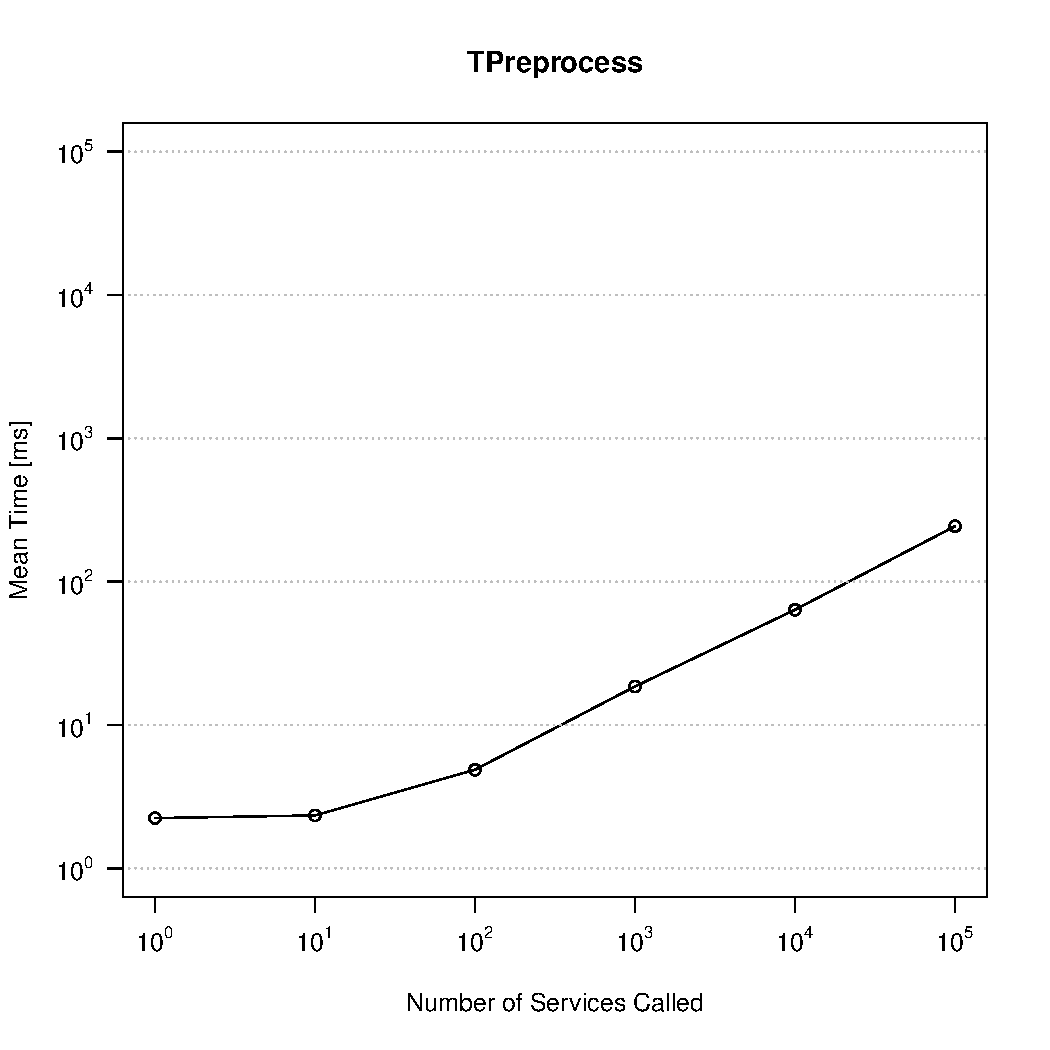
\includegraphics[scale=0.7]{Grafiken/TPreprocess_equal_events_ms.pdf}
\end{figure}
For this test set up $\mathbf{c}$ and $\mathbf{o}$ have a fixed size, but still have to be parsed once each time TPreprocess is called, while $mc$ grows linearly. This results in an complexity of $\mathbf{O(mc * (c + o))}$.

\subsection{x\_different\_events\_one\_user:}
\begin{figure}[H]
	\centering
	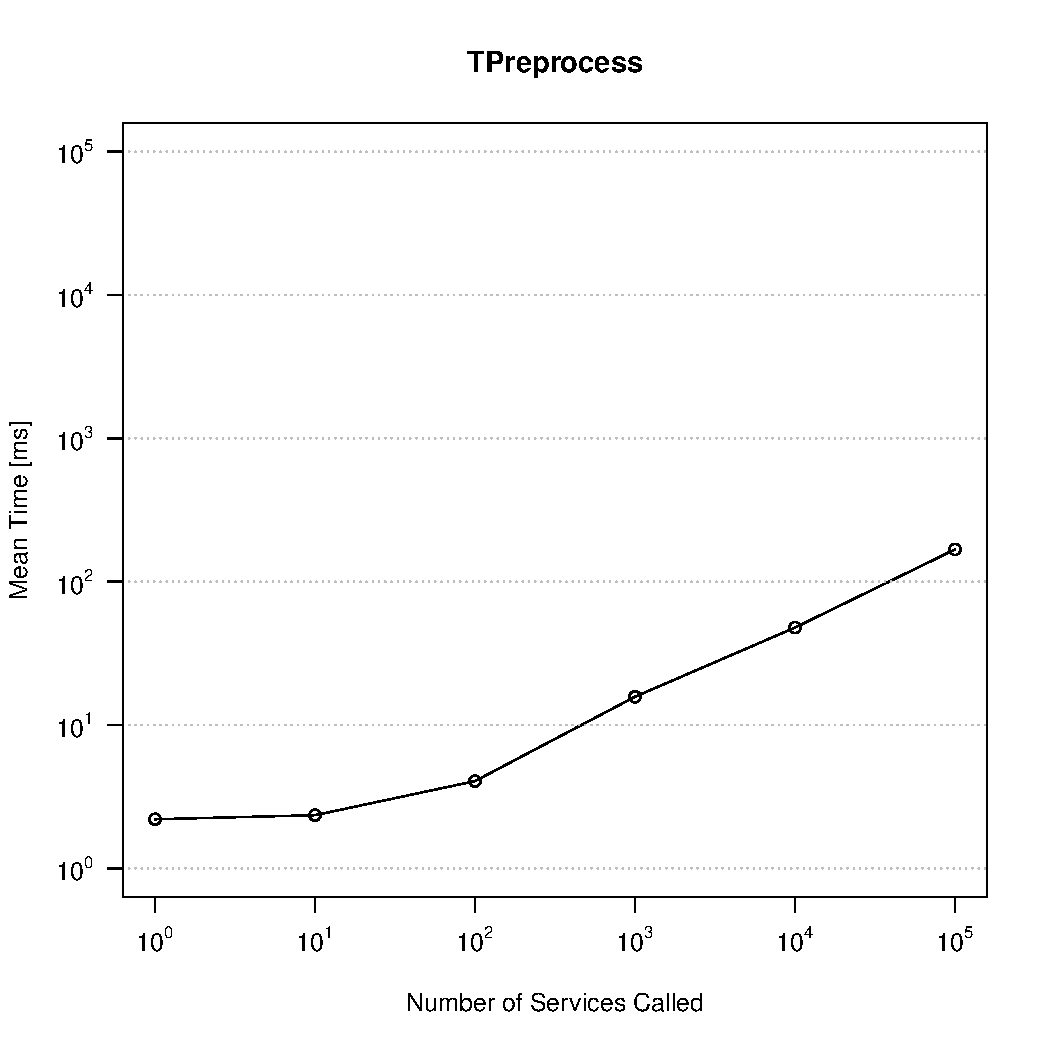
\includegraphics[scale=0.7]{Grafiken/TPreprocess_different_events_ms.pdf}
\end{figure}
For this test set up $\mathbf{c}$ and $\mathbf{o}$ vary, while $\mathbf{mc}$ grows linearly. This overall still results in a complexity of $\mathbf{O(mc * (c + o))}$.

\section{TRuntimeUpdate (TEntryEventSequence):}
This filter loads the PCM UsageModel, uses the incoming EntryCallSequenceModel to do a UserBehaviourTransformation and writes the resulting PCM UsageModel to the disk. As times for loading and writing may vary depending on the underlying system and current use of the disk, only the UserBehaviourTransformation is regarded by this evaluation.\\
\\
The TRuntimeUpdate filter is only called \textbf{once} for each evaluation setup.\\
\\
The complexity of this UserBehaviourTransformation is broken down in the following section.

\subsection{Breakdown of user behaviour transformation}
The time complexity of the usage behaviour transformation is made up of the following parts:

\paragraph{Clustering:}
For the clustering of user groups first a list of distinct operation signatures are extracted from the received EntryCallSystemModel ($O(n*E(n) + n)$). Than each UserSession is transformed a model representing counts of distinct calls of the UserSession ($O((n^2)*E(n))$). This model is than clustered using the xMeansClustering ($O((n+2) * m + 5 * k * n * m)$). Each resulting cluster is than treated as a individual EntryCallSequenceModel ($O(2 * k * n)$).\\
Resulting in an overall complexity of \\$\mathbf{O(E(n) * (n^2 + n) + n + n^2 * m * k + 5 * k * n * m)}$.
\paragraph{Branching:} 
For each created EntryCallSequenceModel, a tree structure called branch model is created, by aggregating the contained EntryCalls ($O(n * log(n) + n * E(n) * (b * log(b) + b))$). Iterating over the tree, the likelihood of occurrence for each branch is calculated ($O(b)$). After that the branch model is compacted, by combining branches with equal ends, removing any unnecessary redundant branch behaviour ($O((S(b) * b)^2 * b * b) $).\\
Resulting in an overall complexity of \\$\mathbf{O(n * log(n) + n * E(n) * (b * log(b) + b) + b + (S(b) * b)^2 * b^2)}$.

\paragraph{Loop detection:}
To find branch behaviour which is actually looped, the branch tree has to be iterated recursively multiple times for each branch.\\
This results in an overall complexity of \\$\mathbf{O(B * S(b)^3 * L(b) * b^2)}$.

\paragraph{Model build:} 
To build a new UsageModel, the created branch model with loops is iterated fully, creating the usage elements.\\
Resulting in an overall complexity of \\$\mathbf{O(B * b * (S(b) + L(b)))}$.\\
\newpage
\paragraph{Combined:}
Adding up and mathematically transforming the time complexities of the four parts results in a combined complexity of:\\
$\mathbf{O(b^4 S(b)^2 + b^2 B K(b) S(b)^3 + b B K(b) + b B S(b) + b n E(n) + }$\\$\mathbf{b n log(b) E(n) + b + n^2 E(n) + n E(n) + k m n^2 + k m n + n + n log(n))}$\\
n = Amount of UserSessions, E(n) = Amount of EntryCallEvents of session n, \\
m = Amount of distinct operation signatures, k = Amount of clusters, \\
b = Amount of Branches, S(b) = Amount of sequence elements of branch b, \\
L(b) = Size of loop in branch b,\\
B = Number of branch models (behaviour transformation internal, corresponds to number of UserGroups)

\subsection{equal\_events\_x\_users:}
\begin{figure}[H]
	\centering
	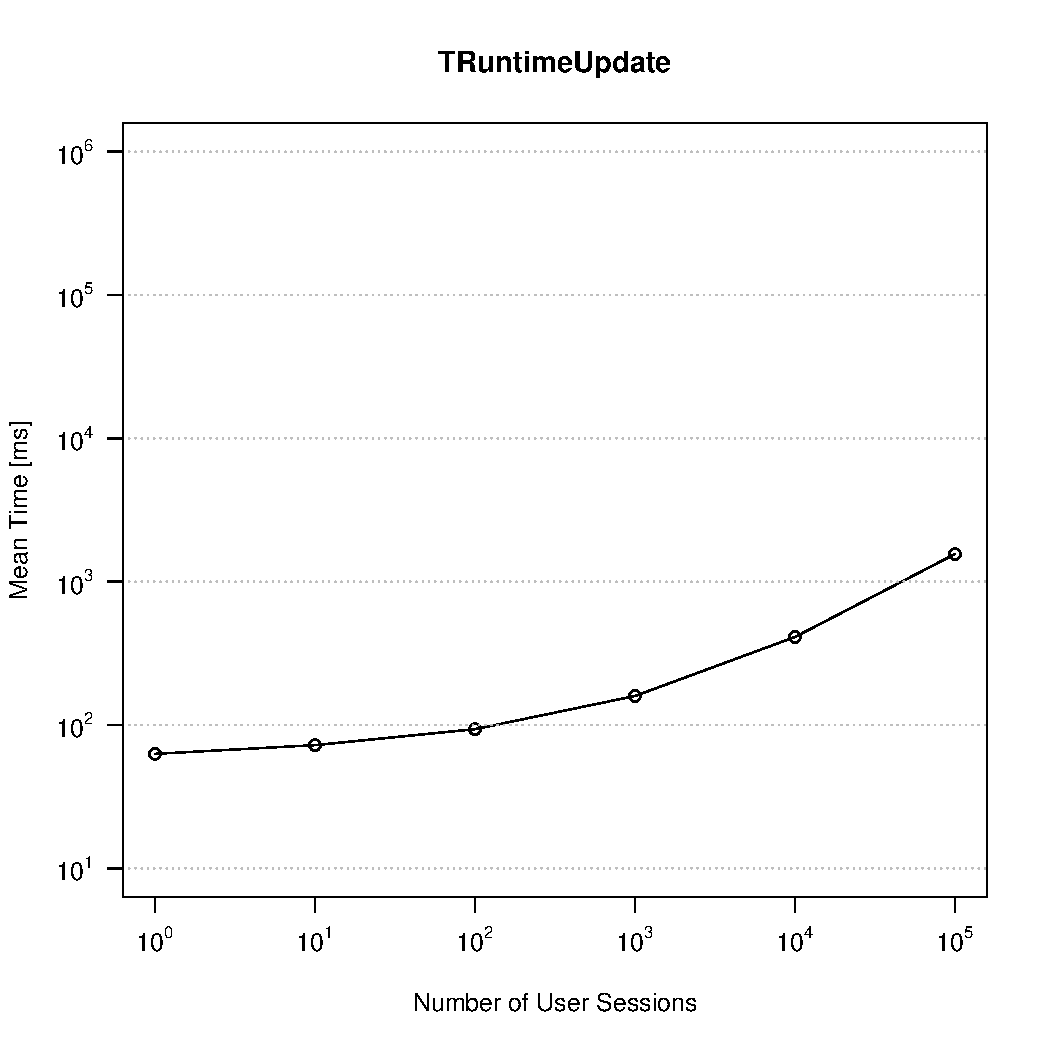
\includegraphics[scale=0.7]{Grafiken/TRuntimeUpdate_equal_events.pdf}
\end{figure}
For this test set up $\mathbf{E(n) = 1, m = 1, k = 1, b = 1, S(b) = 3, L(b) = 0, B = 1}$, while $\mathbf{n}$ grows linearly. Applying this to the general time complexities from above results in the following complexities:\\
Clustering: $\mathbf{O(2 * (n^2) + 7 * n) \rightarrow O(2 * (n^2) + n)}$\\
Branching: $\mathbf{O(n * log(n) + n + 10) \rightarrow O(n * log(n) + n)}$\\
Loop detection: $\mathbf{O(27) \rightarrow O(1)}$\\
Model build: $\mathbf{O(3) \rightarrow O(1)}$\\
\\
Combined: $\mathbf{O(2 * n^2 + 2n + n * log(n))}$\\

\subsection{x\_different\_events\_one\_user:}
\begin{figure}[H]
	\centering
	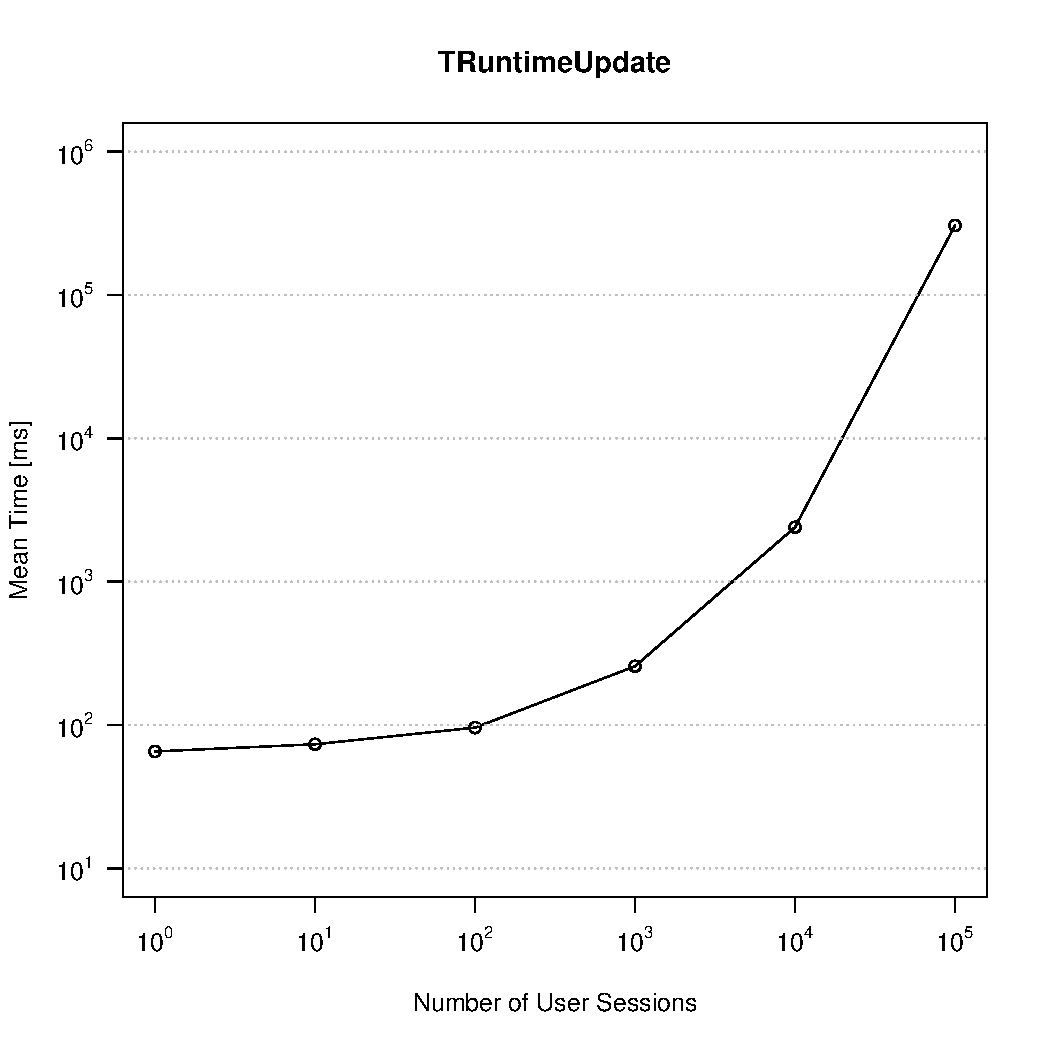
\includegraphics[scale=0.7]{Grafiken/TRuntimeUpdate_different_events.pdf}
\end{figure}
For this test set up $\mathbf{n = 1, m = 13, k = 1, b = 1, B = 1}$, while $\mathbf{E(n)}$ and $\mathbf{S(b)}$ grow linearly. Applying this to the general time complexities from above results in the following complexities:\\
Clustering: $\mathbf{O(E(n) + 79) \rightarrow O(E(n))}$\\
Branching: $\mathbf{O(E(n) + S(b)^2 + 1) \rightarrow O(E(n) + S(b)^2)}$\\
Loop detection: $\mathbf{O(S(b)^3 * L(b))}$\\
Model build: $\mathbf{O(S(b) + L(b))}$\\
\\
Combined: $\mathbf{O(L(b) * S(b)^3 + S(b)^2 + 2 * E(n) + S(b) + L(b))}$\\
\\
The loop detection takes up more than 90\% of the required time. This mostly corresponds to its complexity, when compared to the complexity of the other steps. Still, looking at the logging data, the clustering and branching are much lower than they should be compared to the complexity statements above. It is possible that for this one-sided scenario, with only one big user session, the branching (and also clustering) algorithm can skip most of the time consuming steps, which is not considered in the big O notation.
\end{document}